\documentclass[12pt]{beamer}\usepackage[]{graphicx}\usepackage[]{color}
%% maxwidth is the original width if it is less than linewidth
%% otherwise use linewidth (to make sure the graphics do not exceed the margin)
\makeatletter
\def\maxwidth{ %
  \ifdim\Gin@nat@width>\linewidth
    \linewidth
  \else
    \Gin@nat@width
  \fi
}
\makeatother

\definecolor{fgcolor}{rgb}{0.345, 0.345, 0.345}
\newcommand{\hlnum}[1]{\textcolor[rgb]{0.686,0.059,0.569}{#1}}%
\newcommand{\hlstr}[1]{\textcolor[rgb]{0.192,0.494,0.8}{#1}}%
\newcommand{\hlcom}[1]{\textcolor[rgb]{0.678,0.584,0.686}{\textit{#1}}}%
\newcommand{\hlopt}[1]{\textcolor[rgb]{0,0,0}{#1}}%
\newcommand{\hlstd}[1]{\textcolor[rgb]{0.345,0.345,0.345}{#1}}%
\newcommand{\hlkwa}[1]{\textcolor[rgb]{0.161,0.373,0.58}{\textbf{#1}}}%
\newcommand{\hlkwb}[1]{\textcolor[rgb]{0.69,0.353,0.396}{#1}}%
\newcommand{\hlkwc}[1]{\textcolor[rgb]{0.333,0.667,0.333}{#1}}%
\newcommand{\hlkwd}[1]{\textcolor[rgb]{0.737,0.353,0.396}{\textbf{#1}}}%
\let\hlipl\hlkwb

\usepackage{framed}
\makeatletter
\newenvironment{kframe}{%
 \def\at@end@of@kframe{}%
 \ifinner\ifhmode%
  \def\at@end@of@kframe{\end{minipage}}%
  \begin{minipage}{\columnwidth}%
 \fi\fi%
 \def\FrameCommand##1{\hskip\@totalleftmargin \hskip-\fboxsep
 \colorbox{shadecolor}{##1}\hskip-\fboxsep
     % There is no \\@totalrightmargin, so:
     \hskip-\linewidth \hskip-\@totalleftmargin \hskip\columnwidth}%
 \MakeFramed {\advance\hsize-\width
   \@totalleftmargin\z@ \linewidth\hsize
   \@setminipage}}%
 {\par\unskip\endMakeFramed%
 \at@end@of@kframe}
\makeatother

\definecolor{shadecolor}{rgb}{.97, .97, .97}
\definecolor{messagecolor}{rgb}{0, 0, 0}
\definecolor{warningcolor}{rgb}{1, 0, 1}
\definecolor{errorcolor}{rgb}{1, 0, 0}
\newenvironment{knitrout}{}{} % an empty environment to be redefined in TeX

\usepackage{alltt}
\usepackage{tikz}

% make it pretty
% get rid of junk
\usetheme{default}
\usefonttheme[onlymath]{serif}
\beamertemplatenavigationsymbolsempty

% define a bunch of colors
\definecolor{offwhite}{RGB}{255,250,240}
\definecolor{gray}{RGB}{155,155,155}
\definecolor{foreground}{RGB}{80,80,80}
\definecolor{background}{RGB}{255,255,255}
%\definecolor{title}{RGB}{255,199,0}
\definecolor{title}{RGB}{89,132,212}
%\definecolor{subtitle}{RGB}{89,132,212}
\definecolor{subtitle}{RGB}{255,199,0}
\definecolor{hilit}{RGB}{248,117,79}
\definecolor{vhilit}{RGB}{255,111,207}
\definecolor{lolit}{RGB}{200,200,200}
\definecolor{lit}{RGB}{255,199,0}
\definecolor{mdlit}{RGB}{89,132,212}
\definecolor{link}{RGB}{248,117,79}

% a few color macros
\newcommand{\hilit}{\color{hilit}}
\newcommand{\vhilit}{\color{vhilit}}
\newcommand{\lit}{\color{lit}}
\newcommand{\mdlit}{\color{mdlit}}
\newcommand{\lolit}{\color{lolit}}

% use those colors
\setbeamercolor{titlelike}{fg=title}
\setbeamercolor{subtitle}{fg=subtitle}
\setbeamercolor{frametitle}{fg=gray}
%\setbeamercolor{structure}{fg=subtitle}
\setbeamercolor{structure}{fg=title}
\setbeamercolor{institute}{fg=lolit}
\setbeamercolor{normal text}{fg=foreground,bg=background}
\setbeamertemplate{itemize subitem}{{\textendash}}
\setbeamerfont{itemize/enumerate subbody}{size=\small}
\setbeamerfont{itemize/enumerate subitem}{size=\small}

% center title of slides
\setbeamertemplate{blocks}[rounded]
\setbeamertemplate{frametitle}[default][center]

% page number
\setbeamerfont{page number in foot}{size=\footnotesize}
\setbeamertemplate{footline}[frame number]

% default link color
\hypersetup{colorlinks, urlcolor={link}}

% a few macros
\newcommand{\code}[1]{\texttt{#1}}
\newcommand{\hicode}[1]{{\hilit \texttt{#1}}}
\newcommand{\locode}[1]{{\lolit \texttt{#1}}}
\newcommand{\bb}[1]{\begin{block}{#1}}
\newcommand{\eb}{\end{block}}
\newcommand{\bi}{\begin{itemize}}
\newcommand{\bbi}{\vspace{4pt} \begin{itemize} \itemsep8pt}
\newcommand{\ei}{\end{itemize}}
\newcommand{\bv}{\begin{verbatim}}
\newcommand{\ev}{\end{verbatim}}
\newcommand{\ig}{\includegraphics}
\newcommand{\subt}[1]{{\footnotesize \color{subtitle} {#1}}}
\newcommand{\ttsm}{\tt \small}
\newcommand{\ttfn}{\tt \footnotesize}
\newcommand{\figh}[2]{\centerline{\includegraphics[height=#2\textheight]{#1}}}
\newcommand{\figw}[2]{\centerline{\includegraphics[width=#2\textwidth]{#1}}}



%------------------------------------------------

\title{Visualization Basics}
\subtitle{Intro to Data Visualization}
\author{\href{http://www.gastonsanchez.com}{Gaston Sanchez}}
\institute{\href{https://creativecommons.org/licenses/by-sa/4.0/}{\tt \scriptsize \color{foreground} CC BY-SA 4.0}}
\date{}
\IfFileExists{upquote.sty}{\usepackage{upquote}}{}
\begin{document}



% no page number in first slide
{
  \setbeamertemplate{footline}{} 
  \frame{\titlepage} 
}

%------------------------------------------------

\begin{frame}
\begin{center}
\Huge{\hilit{Vision}}
\end{center}
\end{frame}

%------------------------------------------------

\begin{frame}
\frametitle{Data Visualization?}

\Large Data visualization is simply {\mdlit \textbf{mapping data}} to {\hilit \textbf{geometric objects}}
and their {\lit \textbf{visual attributes}}.

\end{frame}

%------------------------------------------------

\begin{frame}[fragile]
\frametitle{Star Wars data set}

\begin{knitrout}\scriptsize
\definecolor{shadecolor}{rgb}{0.969, 0.969, 0.969}\color{fgcolor}\begin{kframe}
\begin{verbatim}
             name  gender  height  weight      jedi  species      weapon
1  Luke Skywalker    male    1.72      77  yes_jedi    human  lightsaber
2     Leia Organa  female    1.50      49   no_jedi    human     blaster
3  Obi-Wan Kenobi    male    1.82      77  yes_jedi    human  lightsaber
4        Han Solo    male    1.80      80   no_jedi    human     blaster
5           R2-D2    male    0.96      32   no_jedi    droid     unarmed
6           C-3PO    male    1.67      75   no_jedi    droid     unarmed
7            Yoda    male    0.66      17  yes_jedi     yoda  lightsaber
8       Chewbacca    male    2.28     112   no_jedi  wookiee   bowcaster
\end{verbatim}
\end{kframe}
\end{knitrout}

\end{frame}

%------------------------------------------------

\begin{frame}[fragile]
\frametitle{}

\begin{knitrout}\footnotesize
\definecolor{shadecolor}{rgb}{0.969, 0.969, 0.969}\color{fgcolor}

{\centering 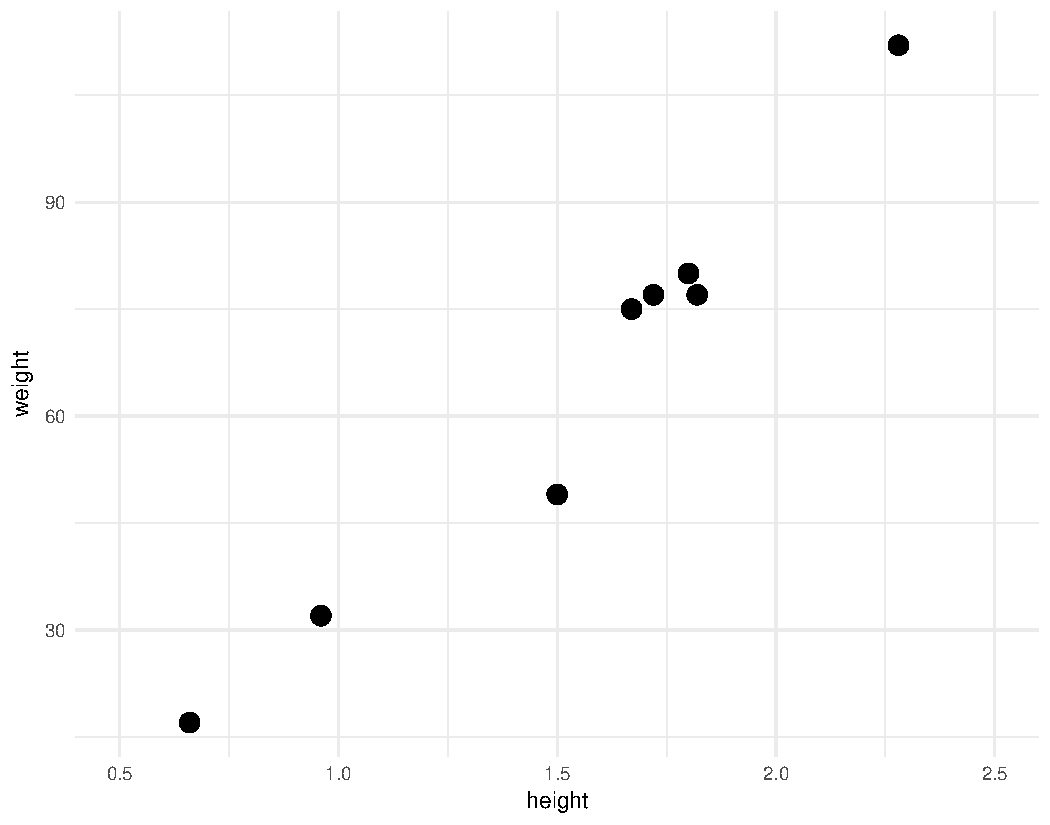
\includegraphics[width=\maxwidth]{figure/scatterplot1-1} 

}



\end{knitrout}

\end{frame}

%------------------------------------------------

\begin{frame}[fragile]
\frametitle{}

\begin{knitrout}\footnotesize
\definecolor{shadecolor}{rgb}{0.969, 0.969, 0.969}\color{fgcolor}

{\centering 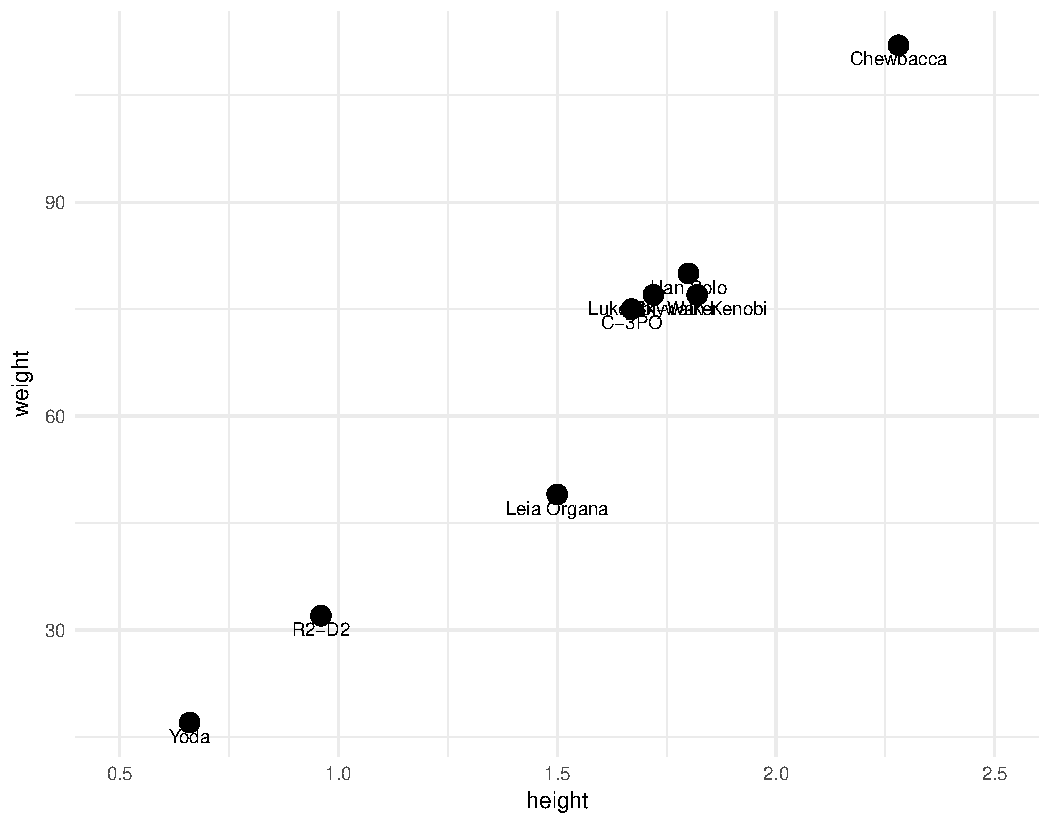
\includegraphics[width=\maxwidth]{figure/scatterplot2-1} 

}



\end{knitrout}

\end{frame}

%------------------------------------------------

\begin{frame}[fragile]
\frametitle{}

\begin{knitrout}\footnotesize
\definecolor{shadecolor}{rgb}{0.969, 0.969, 0.969}\color{fgcolor}

{\centering 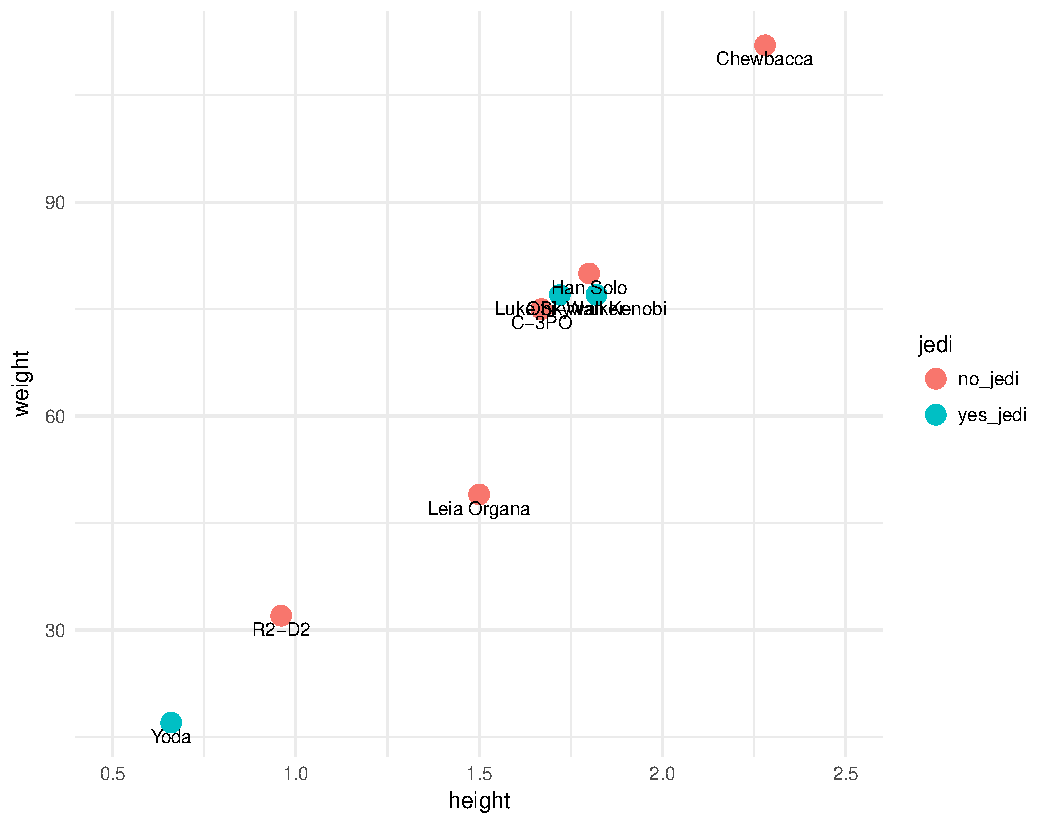
\includegraphics[width=\maxwidth]{figure/scatterplot3-1} 

}



\end{knitrout}

\end{frame}

%------------------------------------------------

\begin{frame}
\frametitle{}

\Large How does it {\lolit (conceptually)} work?

\end{frame}

%------------------------------------------------

\begin{frame}
\begin{center}
\ig[height=8cm]{images/how-does-it-work.pdf}
\end{center}
\end{frame}

%------------------------------------------------

\begin{frame}
\frametitle{Building a Scatterplot}

\bbi
  \item \textbf{Dataset}: starwars
  \item \textbf{Variables}: height, weight, jedi
  \item \textbf{Geometric objects}: points
  \item \textbf{Visual attributes}:
  \bi
    \item X-axis: height, Y-axis: weight
    \item Shape: dots
    \item Color: based on jedi categories
  \ei
\ei

\end{frame}

%------------------------------------------------

\begin{frame}
\frametitle{Mapping Data}
\begin{center}
\ig[width=11cm]{images/mapping-data.pdf}
\end{center}
\end{frame}

%------------------------------------------------

\begin{frame}
\frametitle{Supporting Elements}

\bbi
  \item Axis labels
  \item Legends (positions, labels, symbols)
  \item Choice of colors for points
  \item Background color (i.e. gray)
  \item Grid lines (major and minor)
  \item Axis tick marks
\ei

\end{frame}

%------------------------------------------------

\begin{frame}
\frametitle{In Summary}

\bbi
  \item Graphs consist of several components
  \item Some components represent quantitative values (e.g. lines, bars, etc.)
  \item Some represent categorical values (e.g. color, shape, orientation)
  \item Some play a supporting role (e.g. grid lines, legends, scales on axes)
\ei

\end{frame}

%------------------------------------------------

\begin{frame}
\begin{center}
\Huge{\hilit{Geometric Objects and \\ their Visual Attributes}}
\end{center}
\end{frame}

%------------------------------------------------

\begin{frame}
\frametitle{Mapping Fundamentals}
\begin{center}
\ig[width=9cm]{images/mapping-fundamentals.pdf}
\end{center}
\end{frame}

%------------------------------------------------

\begin{frame}
\frametitle{Geometric Objects (primitives)}
\begin{center}
\ig[width=9cm]{images/geometric-objects.pdf}
\end{center}
\end{frame}

%------------------------------------------------

\begin{frame}
\frametitle{Example of Graphs with Geometric Objects}
\begin{center}
\ig[width=10cm]{images/geometric-objects-examples.pdf}
\end{center}
\end{frame}

%------------------------------------------------

\begin{frame}
\frametitle{ Geometric objects}

Graphical objects (typically) used to encode quantitative values

\bbi
  \item Points
  \item Lines
  \item Bars
  \item 2D areas and polygons
\ei

\end{frame}

%------------------------------------------------

\begin{frame}
\frametitle{Visual Attributes}
\begin{center}
\ig[width=9cm]{images/visual-attribs1.pdf}
\end{center}
\end{frame}

%------------------------------------------------

\begin{frame}
\frametitle{Visual Attributes}
\begin{center}
\ig[width=9cm]{images/visual-attribs2.pdf}
\end{center}
\end{frame}

%------------------------------------------------

\begin{frame}
\frametitle{Visual Attributes of Geometric objects}

Used to encode both quantitative and categorical

\bbi
  \item Position
  \item Color
  \item Size
  \item Shape
  \item Fill pattern
  \item Border
  \item Line style
\ei

\end{frame}

%------------------------------------------------

\begin{frame}
\frametitle{Examples of Visual Attributes}
\begin{center}
\ig[width=7cm]{images/visual-attribs-examples.pdf}
\end{center}
\end{frame}

%------------------------------------------------

\begin{frame}
\begin{center}
{\Huge \hilit{Gallery of Charts}} \\
{\hilit (off-the-self examples)}
\end{center}
\end{frame}

%------------------------------------------------

\begin{frame}
\frametitle{Examples from Google Charts}
\begin{center}
\ig[width=11cm]{images/gallery-google1.pdf}
\end{center}
\end{frame}

%------------------------------------------------

\begin{frame}
\frametitle{Examples from Google Charts}
\begin{center}
\ig[width=11cm]{images/gallery-google2.pdf}
\end{center}
\end{frame}

%------------------------------------------------

\begin{frame}
\frametitle{Examples from Google Charts}
\begin{center}
\ig[width=11cm]{images/gallery-google3.pdf}
\end{center}
\end{frame}

%------------------------------------------------

\begin{frame}
\frametitle{Examples from MS Excel}
\begin{center}
\ig[height=7cm]{images/gallery-excel1.pdf}
\end{center}
\end{frame}

%------------------------------------------------

\begin{frame}
\frametitle{Examples from MS Excel}
\begin{center}
\ig[width=11cm]{images/gallery-excel2.pdf}
\end{center}
\end{frame}

%------------------------------------------------

\begin{frame}
\frametitle{Examples from MS Excel}
\begin{center}
\ig[width=11cm]{images/gallery-excel3.pdf}
\end{center}
\end{frame}

%------------------------------------------------

\begin{frame}
\frametitle{Examples from MS Excel}
\begin{center}
\ig[width=10cm]{images/gallery-excel4.pdf}
\end{center}
\end{frame}

%------------------------------------------------

\begin{frame}
\frametitle{Examples from ggplot2}
\begin{center}
\ig[height=7cm]{images/gallery-ggplot1.pdf}
\end{center}
\end{frame}

%------------------------------------------------

\begin{frame}
\frametitle{Examples from ggplot2}
\begin{center}
\ig[width=11cm]{images/gallery-ggplot2.pdf}
\end{center}
\end{frame}

%------------------------------------------------

\begin{frame}
\begin{center}
\Huge{\hilit{So how do you approach graphing data?}}
\end{center}
\end{frame}

%------------------------------------------------

\begin{frame}
\frametitle{Creating graphs \dots}

{\Large
\begin{quotation}
\noindent With computer technology, anyone can create graphics, but few of us know how to do it well.

\bigskip
{\small \noindent \textit{Donna Wong}}

\end{quotation}
}

\end{frame}

%------------------------------------------------

\begin{frame}
\frametitle{Approaching graphing data}

With so many chart options, and various software tools, how can you determine what type of graph should you use?

\bigskip

In my opinion, there are a couple of aspects to always keep in mind:

\bi
  \item Data encoding (core idea )
  \item Common analytical tasks
  \item Visual perception basics
  \item Effective charts suggestions
\ei

\end{frame}

%------------------------------------------------

\begin{frame}
\begin{center}
\Huge{\hilit{Analytical Tasks}}
\end{center}
\end{frame}

%------------------------------------------------

\begin{frame}
\frametitle{}

\Large Following Stephen Few's philosophy, creating charts can be approached from the type of analytical task (or analytical pattern) to be used.

\end{frame}

%------------------------------------------------

\begin{frame}
\frametitle{Approaching graphing data}

\bi
  \item Part-to-whole analysis
  \item Ranking analysis
  \item Deviation analysis
  \item Times series (trends in time)
  \item Distribution analysis
  \item Correlation analysis
  \item Multivariate analysis
\ei

\end{frame}

%------------------------------------------------

\begin{frame}
\frametitle{GSW Game Results (regular season 2017-2018)}
\begin{center}
\ig[width=10cm]{images/gsw-game-results-2018.pdf}
\end{center}
\end{frame}

%------------------------------------------------

\begin{frame}
\frametitle{Pay attention to \dots}

I'll show you some Analytical Task examples using GSW Game Results data. In each graph, pay attention to the following:

\bbi
  \item type of data (quant, categ)
  \item geometric object(s)
  \item visual attribute(s)
  \item supporting elements
\ei



\end{frame}

%------------------------------------------------

\begin{frame}[fragile]
\frametitle{Task: Part-to-whole}

\begin{knitrout}\footnotesize
\definecolor{shadecolor}{rgb}{0.969, 0.969, 0.969}\color{fgcolor}

{\centering 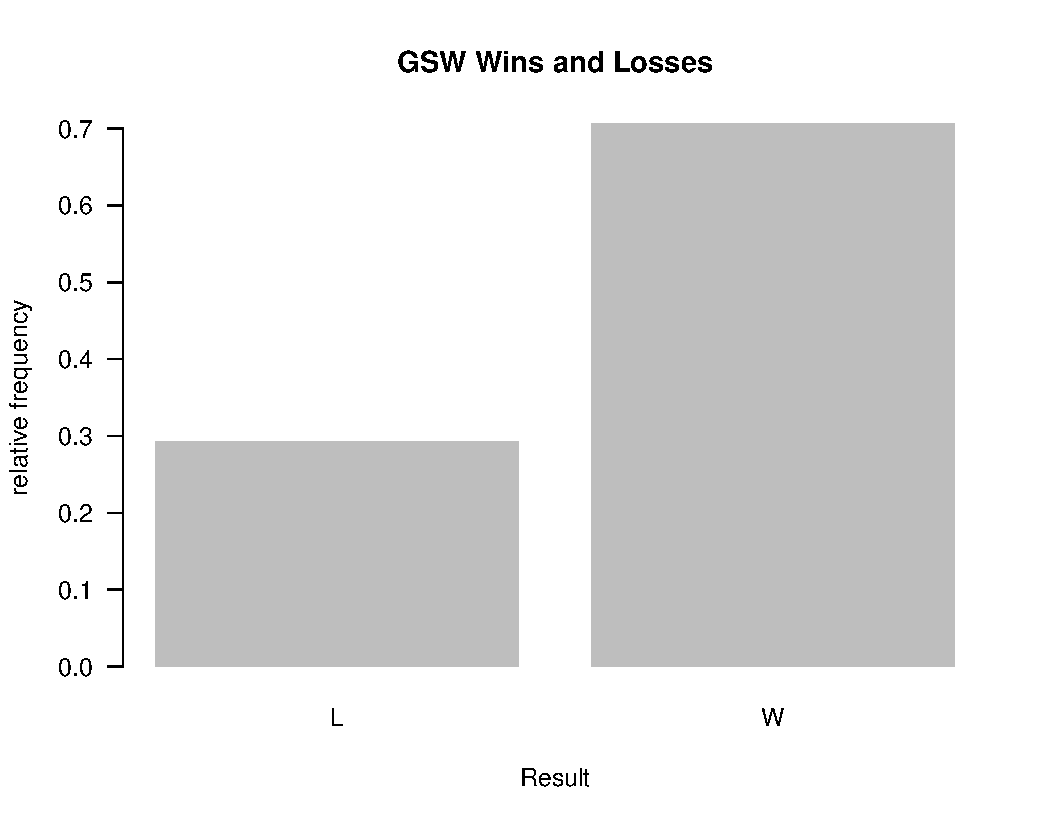
\includegraphics[width=\maxwidth]{figure/task_proportion-1} 

}



\end{knitrout}

\end{frame}

%------------------------------------------------

\begin{frame}[fragile]
\frametitle{Task: Distribution}

\begin{knitrout}\footnotesize
\definecolor{shadecolor}{rgb}{0.969, 0.969, 0.969}\color{fgcolor}

{\centering 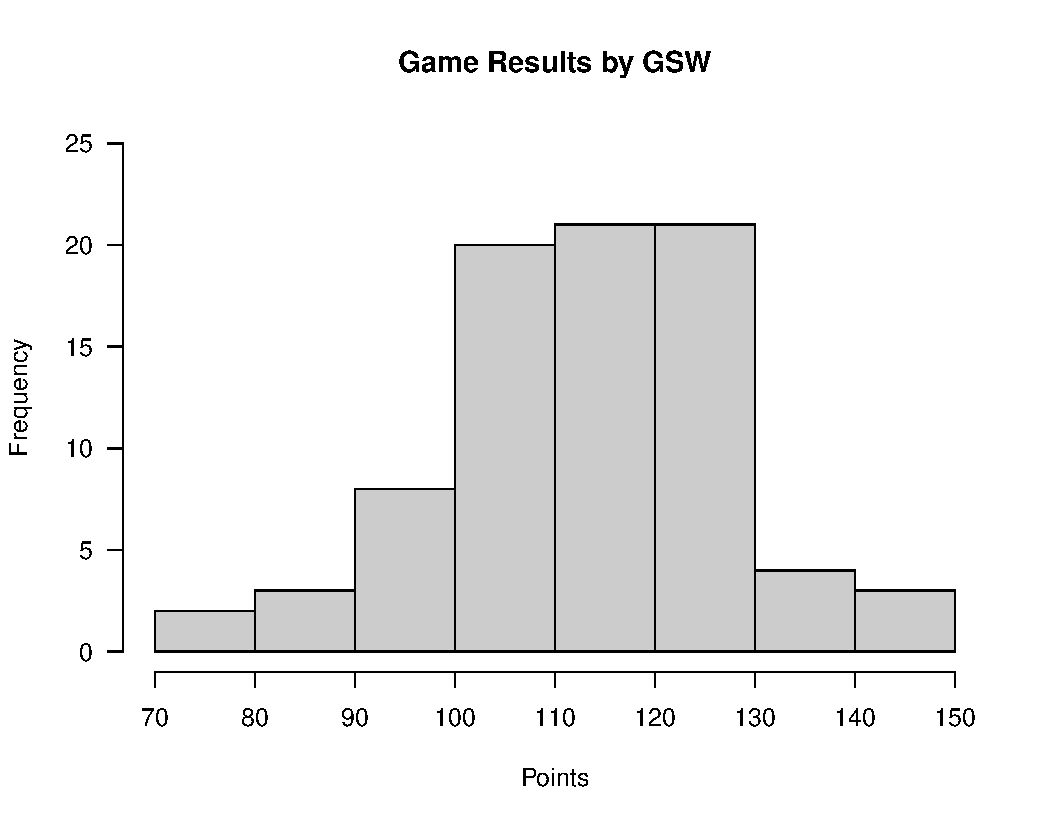
\includegraphics[width=\maxwidth]{figure/task_distrib1-1} 

}



\end{knitrout}

\end{frame}

%------------------------------------------------

\begin{frame}[fragile]
\frametitle{Task: Distribution}

\begin{knitrout}\footnotesize
\definecolor{shadecolor}{rgb}{0.969, 0.969, 0.969}\color{fgcolor}

{\centering 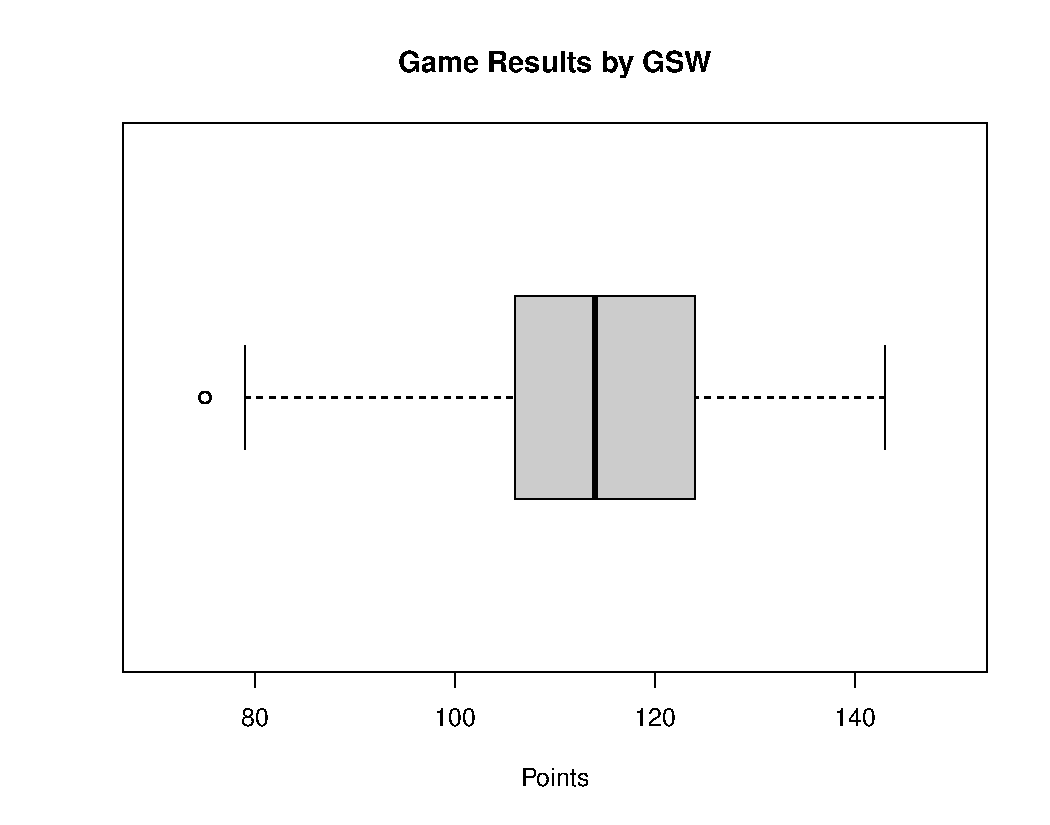
\includegraphics[width=\maxwidth]{figure/task_distrib2-1} 

}



\end{knitrout}

\end{frame}

%------------------------------------------------

\begin{frame}[fragile]
\frametitle{Task: Distribution}

\begin{knitrout}\footnotesize
\definecolor{shadecolor}{rgb}{0.969, 0.969, 0.969}\color{fgcolor}

{\centering 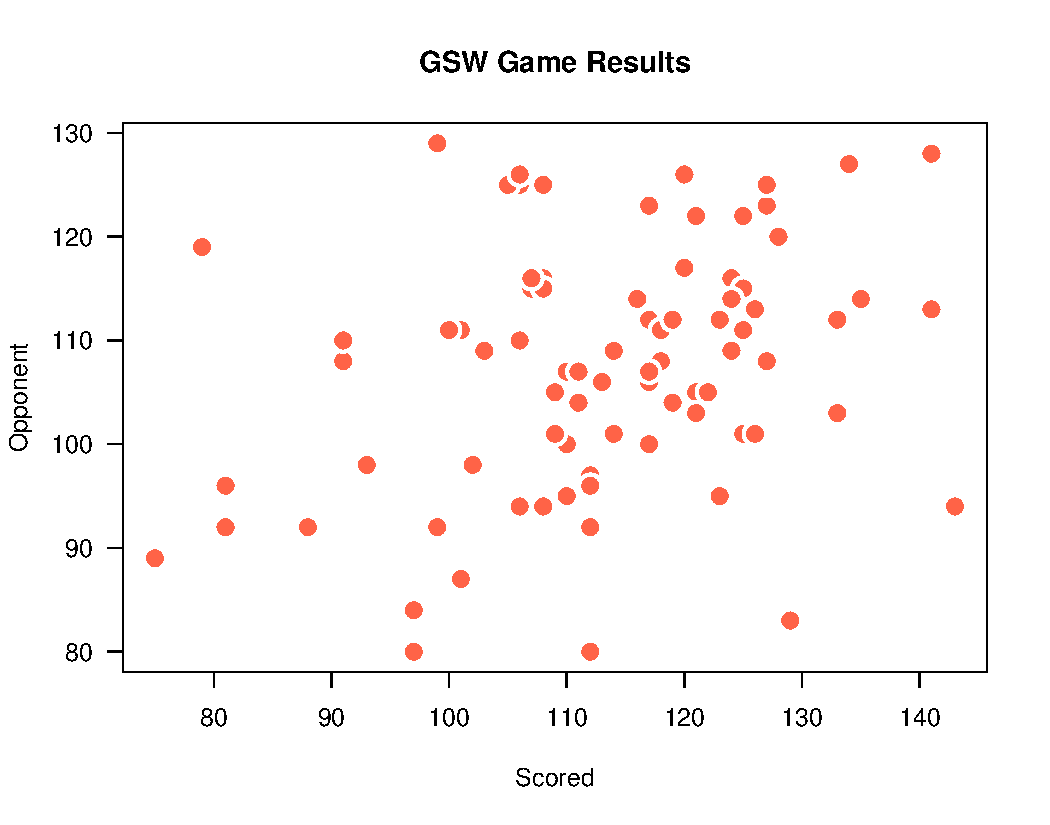
\includegraphics[width=\maxwidth]{figure/task_correlation-1} 

}



\end{knitrout}

\end{frame}

%------------------------------------------------

\begin{frame}[fragile]
\frametitle{Task: Deviation}

\begin{knitrout}\footnotesize
\definecolor{shadecolor}{rgb}{0.969, 0.969, 0.969}\color{fgcolor}

{\centering 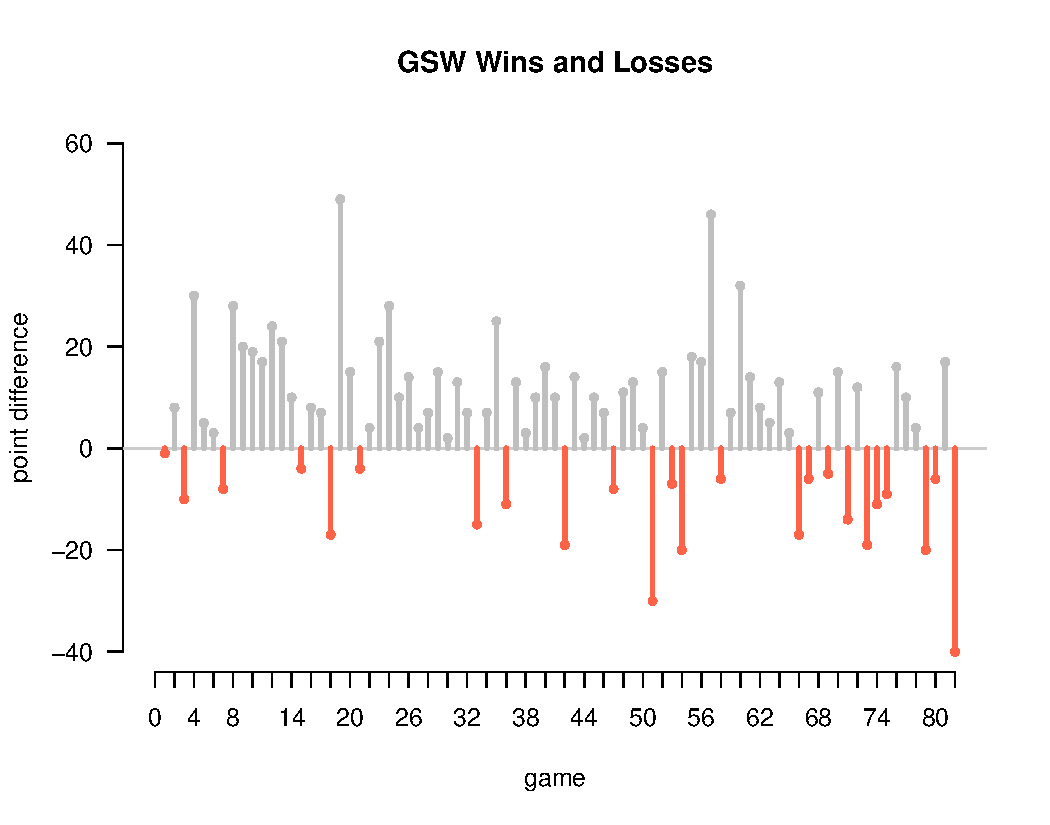
\includegraphics[width=\maxwidth]{figure/task_deviation-1} 

}



\end{knitrout}

\end{frame}

%------------------------------------------------

\begin{frame}[fragile]
\frametitle{Task: Ranking}

\begin{knitrout}\footnotesize
\definecolor{shadecolor}{rgb}{0.969, 0.969, 0.969}\color{fgcolor}

{\centering 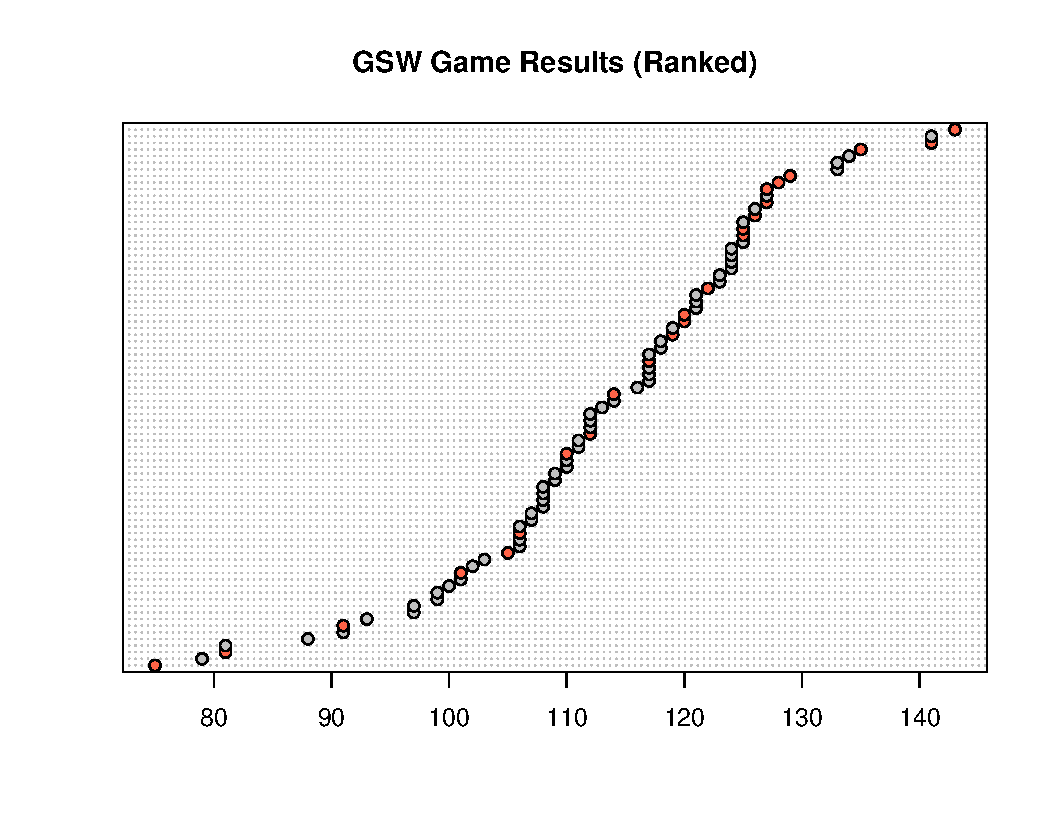
\includegraphics[width=\maxwidth]{figure/task_ranking-1} 

}



\end{knitrout}

\end{frame}

%------------------------------------------------

\begin{frame}[fragile]
\frametitle{Task: Time trend}

\begin{knitrout}\footnotesize
\definecolor{shadecolor}{rgb}{0.969, 0.969, 0.969}\color{fgcolor}

{\centering 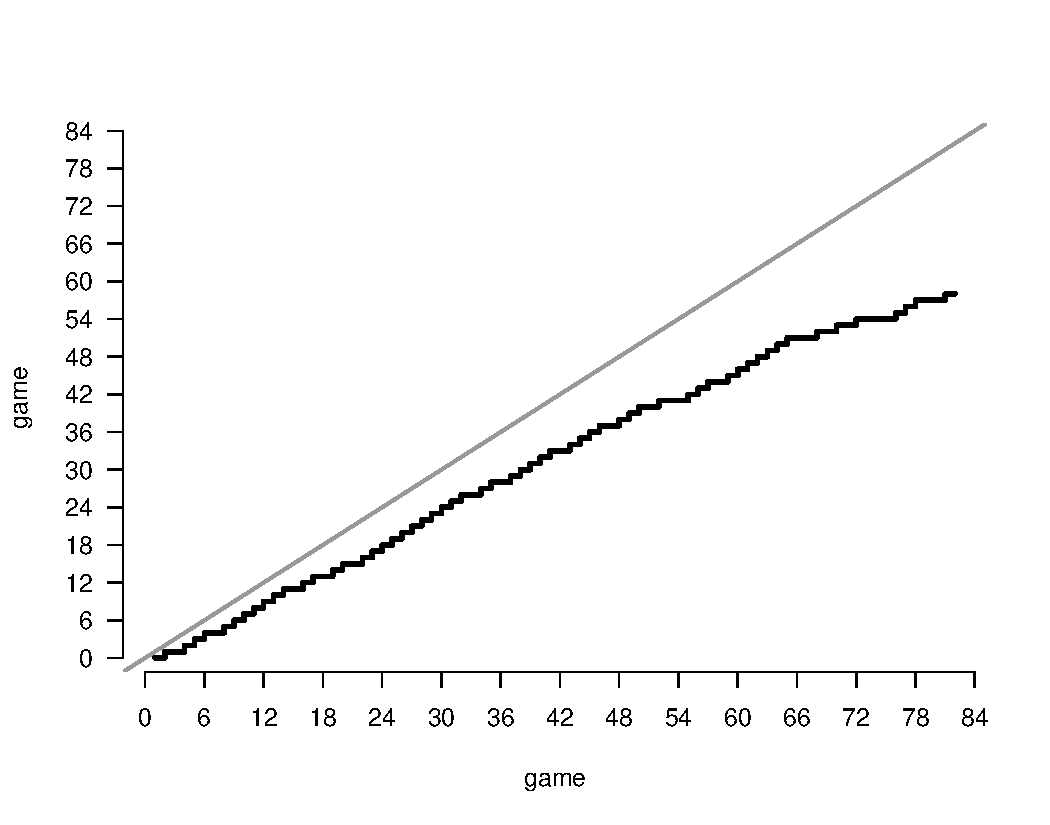
\includegraphics[width=\maxwidth]{figure/task_timeline-1} 

}



\end{knitrout}

\end{frame}

%------------------------------------------------

\begin{frame}
\frametitle{Next}

To create effective data visualizations we also need to briefly talk about how our visual system works, as well as some visual perception aspects related with charts and graphs.

\end{frame}

%------------------------------------------------

\end{document}
